% --------------------------------------------------------------
% This is all preamble stuff that you don't have to worry about.
% Head down to where it says "Start here"
% --------------------------------------------------------------
 
\documentclass[12pt]{article}
 
\usepackage[margin=1in]{geometry} 
\usepackage{amsmath,amsthm,amssymb}
\usepackage{graphicx}
\usepackage[space]{grffile}
\usepackage{subcaption}
\usepackage{float}
\newcommand{\N}{\mathbb{N}}
\newcommand{\Z}{\mathbb{Z}}
\title{Cmpe-537 \\ Computer Vision \\ Assignment-2
}
\author{Abdullah Atakan Guney \\ 2018700069}
\date{November 4, 2018}
\begin{document}
 
\maketitle

\newpage

\tableofcontents

\newpage

\section{Problem}
In this assignment, I developed a image stitching system which can stitch multiple images in order to create a single panoramic image. Program implemented in Python 3.

\section{Image Stitching Procedure}
\subsection{Select Common Points on Images}
As it is told in the description, I have used matplotlib.pyplot.ginput to get corresponding points between images.

\subsection{Homography Estimation}
I calculated $H$ matrix by calculating SVD of matrix $A$ which is given below:

\begin{equation*}
    A = \left[ \begin{array}{ccccccccc}
         x_1 & y_1 & 1 & 0 & 0 & 0 & u_1 x_1 & u_1 y_1 & u_1  \\ 
         0 & 0 & 0 & x_1 & y_1 & 1 & v_1 x_1 & v_1 y_1 & v_1  \\
          &  &  &  & \vdots &  &  &  & \\
         x_N & y_N & 1 & 0 & 0 & 0 & u_N x_N & u_N y_N & u_N  \\ 
         0 & 0 & 0 & x_N & y_N & 1 & v_N x_N & v_N y_N & v_N  \\     
    \end{array} \right]
\end{equation*}

Matrix $A$ holds the equality:

\begin{equation*}
    \left[ \begin{array}{ccccccccc}
         x_1 & y_1 & 1 & 0 & 0 & 0 & u_1 x_1 & u_1 y_1 & u_1  \\ 
         0 & 0 & 0 & x_1 & y_1 & 1 & v_1 x_1 & v_1 y_1 & v_1  \\
          &  &  &  & \vdots &  &  &  & \\
         x_N & y_N & 1 & 0 & 0 & 0 & u_N x_N & u_N y_N & u_N  \\ 
         0 & 0 & 0 & x_N & y_N & 1 & v_N x_N & v_N y_N & v_N  \\     
    \end{array} \right] \times \left[ \begin{array}{c}
         h_1 \\
         h_2 \\
         \vdots \\
         h_{N-1} \\
         h_N
    \end{array}\right] = \mathbf{0}
\end{equation*}

The estimation of $h$ given by singular vector which corresponds to least singular value, so $h \approx V_N$.

I have used numpy's svd algorithm to calculate $h$. Given $h$,
\begin{equation*}
    H = \left[ \begin{array}{ccc}
         h_1 & h_2 & h_3 \\
         h_4 & h_5 & h_6 \\
         h_7 & h_8 & h_9
    \end{array}\right]
\end{equation*}

Additionally, to calculate a robust transformation matrix, I have also normalized all input points before calculate $H$, such that average length of points is $\sqrt{2}$ and average of points is $(0, 0)$.

By given transformation matrix $T_1$ and $T_2$ such that
\begin{align*}
    T_2 x' = H' T_1 x \\
    x' = T_2^{-1} H' T_1 x \\
    H = T_2^{-1} H' T_1
\end{align*}

\subsection{Image Warping}
Image warping is changing the domain of the image function, rather than filtering. Let say we have transformation matrix $H$, which transforms domain of image-1 to the domain of image-2, then warping corresponds to finding $g(x')$. So,

\begin{equation*}
    g(x') = f(H(x))
\end{equation*}
where $f$ is the input image of warping function and $g$ is the output function. There are 2 major methods to calculate output image: Forward and backward transformation. I used backward transformation, which aims to find output image's pixels by transforming its index back to input image by using inverse transformation matrix $H^{-1}$.

\begin{equation*}
    H^{-1} x' = x
\end{equation*}

After finding all corresponding $x$, we can set $g(x)$. But result of inverse transformation can be placed between pixels on input image. So, I have used nearest-neighbour interpolation from "scipy" library.

In this assignment, first I have calculated borders for output image by forward transformation of corner points of input image. Then, I have calculated range for output image. By using $H^{-1}$, I have calculated all the corresponding points of the points in the range calculated, then I have assigned points of output image to corresponding input image pixel.

\subsection{Image Blending}

For blending all the images, first I have transformed the domain of all the images into middle one's domain. Then by warping all these images, I have calculated range for all of these. After all, I merged them into new big image. On the overlapping points, I have used a basic strategy that if overlapping pixel is zero in of the intersecting images, I have used the other one, and if both are non-zero, I used the average of them.

\section{Experiments}
\subsection{Number of Points}
I have experimented on both 5 and 12 corresponding points.

\begin{figure}[H]
    \centering
    \begin{subfigure}{\textwidth}
        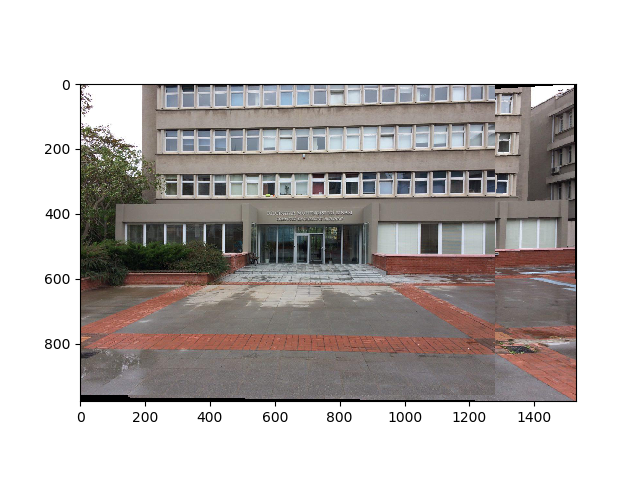
\includegraphics[width=\textwidth, height=0.4\textheight]{figs/5-correspondence.png}
        \caption{Result for 5 correspondence points}
        \label{fig:5points}
    \end{subfigure}
    \begin{subfigure}{\textwidth}
        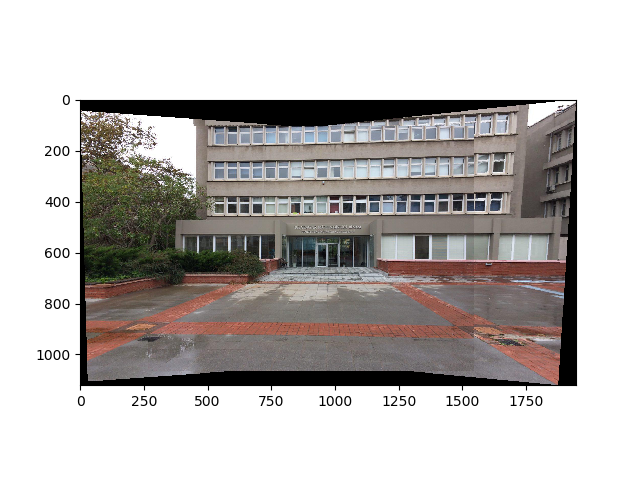
\includegraphics[width=\textwidth, height=0.4\textheight]{figs/12-correspondence.png}
        \caption{Result for 12 correspondence points}
        \label{fig:12points}
    \end{subfigure}
\end{figure}

As we can observe that choosing more correspondence points results better. It is obvious that for above equation 5 points would be enough but more points are resulting better.

\subsection{Point Selection}
\subsubsection{Without Normalization}
\begin{figure}[H]
    \centering
    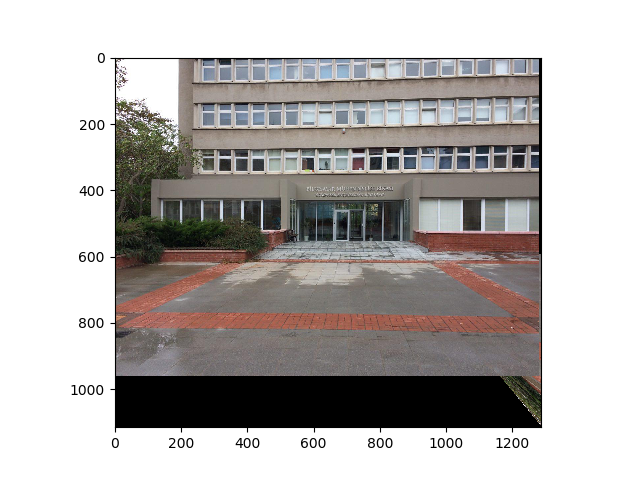
\includegraphics[width=\textwidth, height=0.4\textheight]{figs/12-3-wrong-unnormalized.png}
    \caption{3 wrong points are selected out of 12}
    \label{fig:3-wrong-unnormalized}
\end{figure}

\subsubsection{With Normalization}
\begin{figure}[H]
    \centering
    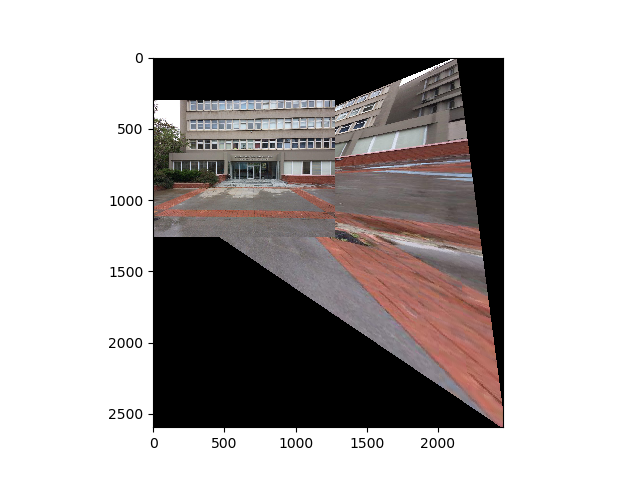
\includegraphics[width=\textwidth, height=0.4\textheight]{figs/12-3-wrong-normalized.png}
    \caption{3 wrong points are selected out of 12}
    \label{fig:3-wrong-normalized}
\end{figure}

\begin{figure}[H]
    \centering
    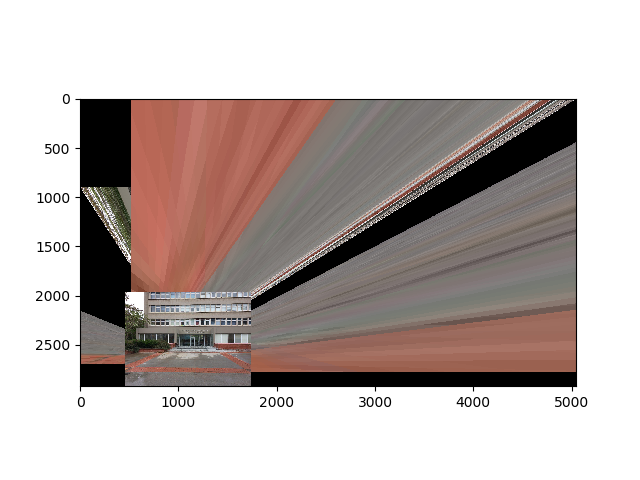
\includegraphics[width=\textwidth, height=0.4\textheight]{figs/12-5-wrong-normalized.png}
    \caption{5 wrong points are selected out of 12}
    \label{fig:5-wrong-normalized}
\end{figure}

As we can see easier, choosing wrong points cause problem, and without normalization, transformation has almost no effect when we select points wrong.

\subsection{Noisy Points}
\subsubsection{Normalized}
\begin{figure}[H]
    \centering
    \begin{subfigure}{\textwidth}
        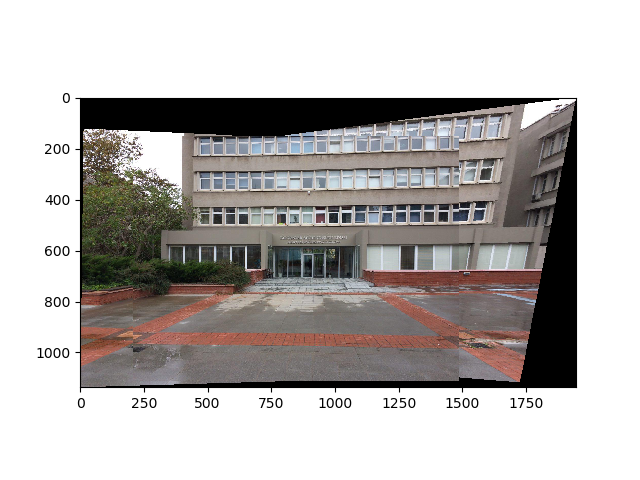
\includegraphics[width=\textwidth,
        height=0.3\textheight]{figs/gaussian-noise-1.png}
        \caption{Gaussian Noise with variance 1}
        \label{fig:gaussian-1}
    \end{subfigure}
    
    \begin{subfigure}{\textwidth}
        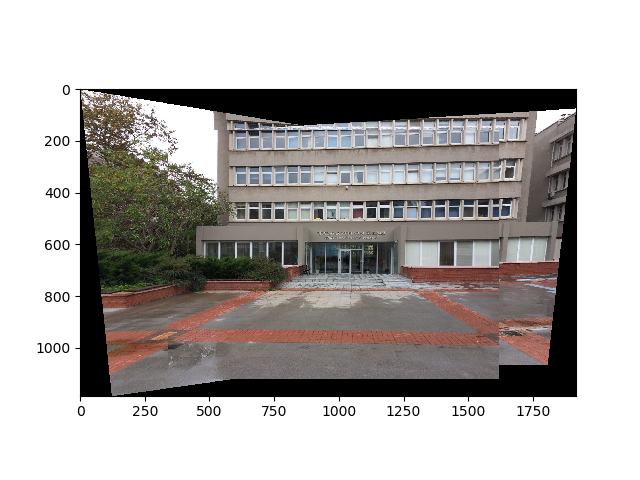
\includegraphics[width=\textwidth,
        height=0.3\textheight]{figs/gaussian-noise-5.png}
        \caption{Gaussian Noise with variance 5}
        \label{fig:gaussian-5}
    \end{subfigure}
    
    \begin{subfigure}{\textwidth}
        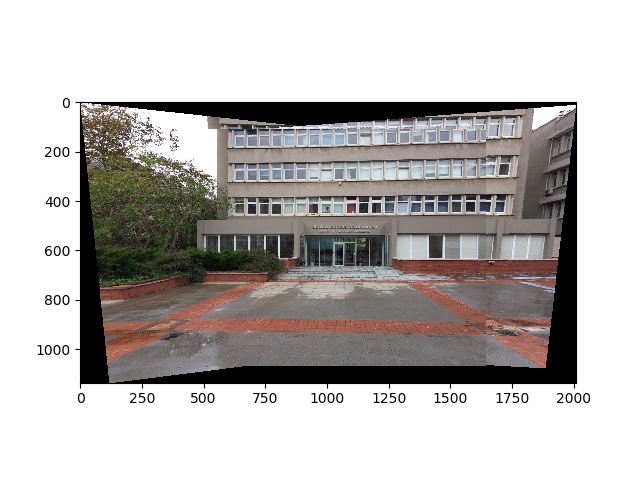
\includegraphics[width=\textwidth,
        height=0.3\textheight]{figs/gaussian-noise-10.png}
        \caption{Gaussian Noise with variance 10}
        \label{fig:gaussian-10}
    \end{subfigure}
\end{figure}

So, as we can observe since normalizing is used, gaussian noise won't be so problematic.

\subsubsection{Unnormalized}
\begin{figure}[H]
    \centering
    \begin{subfigure}{\textwidth}
        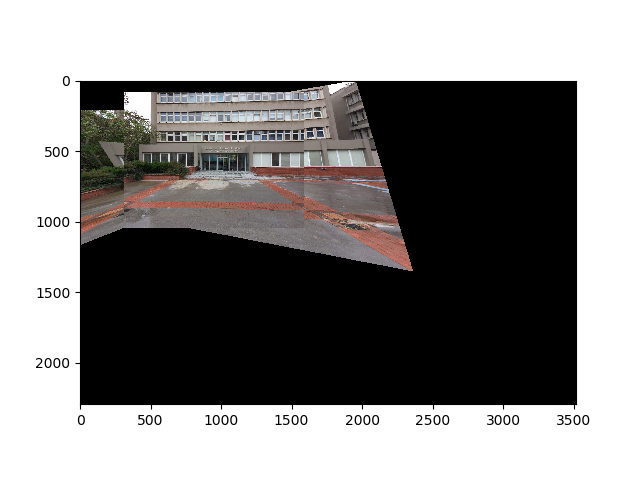
\includegraphics[width=\textwidth,
        height=0.3\textheight]{figs/gaussian-noise-unnormalized-1.png}
        \caption{Gaussian Noise with variance 1}
        \label{fig:gaussian-unnormalized-1}
    \end{subfigure}
    
    \begin{subfigure}{\textwidth}
        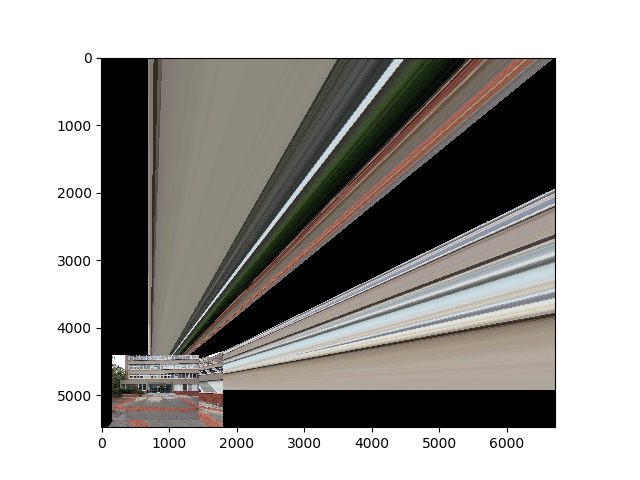
\includegraphics[width=\textwidth,
        height=0.3\textheight]{figs/gaussian-noise-unnormalized-5.png}
        \caption{Gaussian Noise with variance 5}
        \label{fig:gaussian-unnormalized-5}
    \end{subfigure}
\end{figure}

In unnormalized version, Gaussian noise would effect results even with little noise.

\subsection{Stitching All}

I have tried 3 different approach to handle overlapping pixels when blending all five images. In one of them I added images directly but in a natural way that gives priority to the middle image, in the second one, I averaged overlapped pixels, and lastly I set maximum intensity for each color channel. Results follows,

\begin{figure}[H]
    \centering
    \begin{subfigure}{\textwidth}
        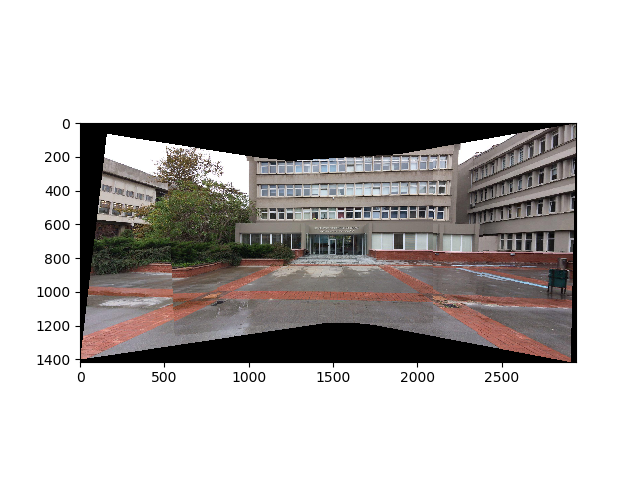
\includegraphics[width=\textwidth,
        height=0.3\textheight]{figs/all-5.png}
        \caption{All images blended directly top of each other}
        \label{fig:all}
    \end{subfigure}
    
    \begin{subfigure}{\textwidth}
        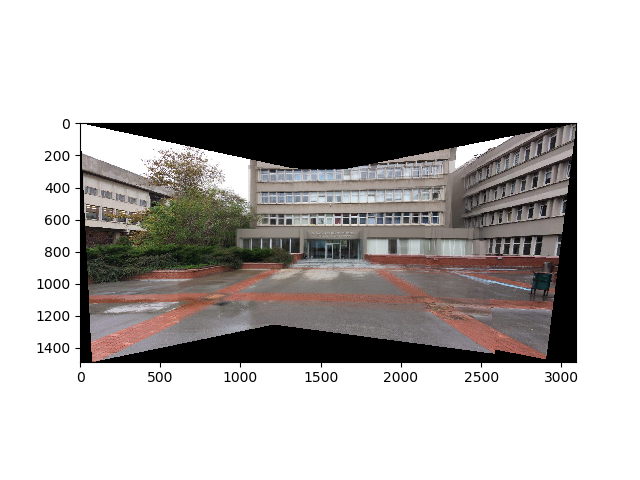
\includegraphics[width=\textwidth,
        height=0.3\textheight]{figs/all-5-avg.png}
        \caption{Overlapping pixels are averaged}
        \label{fig:all-avg}
    \end{subfigure}
    
    \begin{subfigure}{\textwidth}
        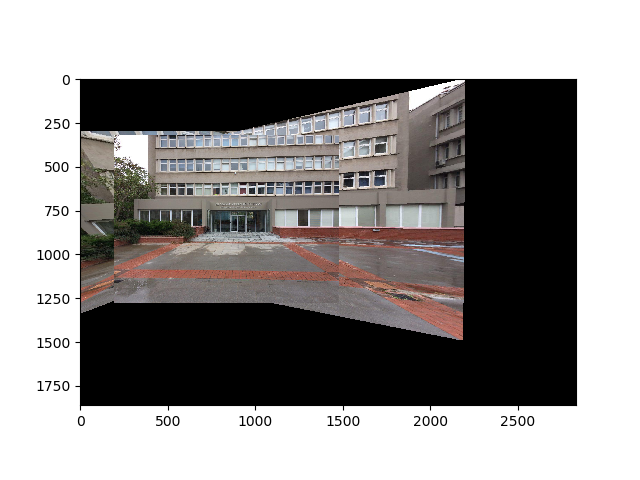
\includegraphics[width=\textwidth,
        height=0.3\textheight]{figs/all-5-max.png}
        \caption{Set it to max intensities}
        \label{fig:all-max}
    \end{subfigure}
\end{figure}

\end{document}